\section{Application: violent crime across U.S. communities}
\label{sec:realdata}

The analysis contains $n=1{,}993$ communities and $p=99$ candidate
predictors. Under the tuning selected in Section~\ref{sec:tuning},
$\alpha=n^{-0.3}\approx0.102$ and $h=n^{-0.15}/2\approx0.160$, so the
sample contains $n\alpha\approx204$ upper-tail observations in total and
about $2n\alpha h\approx65$ within a typical interior rank window. The
dimension is therefore comparable to the number of observations
available for local tail estimation. Unrestricted or nonparametric joint
tail modelling with $99$ covariates is poorly supported by roughly $200$
upper-tail observations, and by fewer still within any local covariate
neighbourhood; a marginal screen can rank the $99$ candidates from
exactly this information.

\subsection{Data and protocol}

The Communities and Crime data set
\citep{redmond2002}, distributed by the UCI Machine Learning Repository
in its unnormalized version, links socio-economic census attributes,
law-enforcement survey attributes and FBI crime counts for $2{,}215$ U.S.
communities. The response is the violent-crime rate per $100{,}000$
inhabitants. We keep the communities with an observed positive response
($n=1{,}993$). Preprocessing of the $124$ documented predictive
attributes is response-blind: we retain numeric predictors with fewer
than $5\%$ missing values, which removes the $22$ law-enforcement
variables reported by only $343$ communities, and with at least $100$
distinct observed values, which removes $3$ low-cardinality variables,
keeping the application close to the continuous-marginal framework of
the theory. This leaves $p=99$ continuous predictors --- demographic
composition, income and poverty, education, employment, family
structure, immigration, language, housing, and population density. The
at most one missing value per retained predictor is median-imputed, and
every method below works from the same imputed matrix.

The response is strongly right-skewed: median $374$, $99$th percentile
$2{,}943$, maximum $4{,}877$. The left panel of Figure~\ref{fig:crime}
shows the Hill curve of the response over $k\in[20,600]$ upper order
statistics; it is positive and moves slowly, between $0.283$ and
$0.374$ for $k\in[100,300]$, with value $0.328$ at the working level
$k=n\alpha=204$. The middle panel shows the Pareto QQ plot of the $600$
largest responses, approximately linear over the working range with
least-squares slope $0.27$. The gap between the QQ slope and the Hill
value at the same level is mild evidence that regular variation is only
approximate over the working range. The response exhibits a
sufficiently heavy and stable upper tail to make a tail-index analysis
plausible; neither diagnostic establishes regular variation beyond
doubt, and no single threshold carries a structural interpretation.

The screening protocol is the one fixed in Section~\ref{sec:tuning},
applied unchanged: the aggregated tail-index screen computes the score
at each of the nine settings
$\mathcal N_9=\{0.30,0.35,0.40\}\times\{0.10,0.15,0.20\}$, converts
each pass into ranks, and orders the predictors by the minimum rank
$r_j^{\rm agg}$ across the nine settings; the selected-pair screen at
$(a^\star,b^\star)=(0.30,0.15)$ is reported alongside. The two
competing screens of Section~\ref{sec:comparison} are run on the same
imputed matrix: Yoshida--Umezu at its transplanted tuning and the
quantile screen at $\tau\in\{.90,.95,.99\}$.

\subsection{Results}

Poverty and family structure dominate the aggregated ranking, and they
dominate every competing ranking as well. The two-parent household
variable \texttt{pctKids2Par} is first (per-setting ranks $1$--$4$
across the nine settings), the poverty rate \texttt{pctPoverty} second
(ranks $1$--$6$) and \texttt{pct2Par} third (ranks $1$--$5$); the two
family-structure variables are also leading variables for the quantile
screen at every level (\texttt{pctKids2Par} is first at all three
$\tau$) and for Yoshida--Umezu (ranks $3$--$7$). The related
\texttt{pctKids4w2Par} and \texttt{pct12to17w2Par} complete the
consensus block at aggregated ranks $7$--$8$. The high-quantile and
tail-index rankings share these leading predictors.

The informative disagreements are the tail-specific candidates. The
share of workers using public transportation
(\texttt{pctUsePubTrans}, aggregated rank $5$) and the farm-employment
rate (\texttt{pctWfarm}, rank $6$) rank far lower under every
fixed-quantile method: ranks $49$--$73$ for the quantile screen across
its three levels and $57$--$60$ for Yoshida--Umezu. Their low
tail-index scores are consistent with marginal variation in upper-tail
heaviness across their values, of a kind that fixed-quantile screens are
not designed to detect; Section~\ref{sec:comparison} produces the same
dissociation under controlled conditions, where the target is known.
The two variables differ in stability across the aggregation block:
\texttt{pctUsePubTrans} ranks within the top $15$ at every one of the
nine settings, while \texttt{pctWfarm} moves between $2$ and $47$
(right panel of Figure~\ref{fig:crime}). The never-married male rate
(\texttt{pctMaleNevMar}, aggregated rank $4$, per-setting ranks
$1$--$9$, quantile ranks $28$--$35$) sits between the consensus block
and the tail-specific pair. We report all three as candidate
tail-specific predictors for a second-stage analysis.

Minimum-rank aggregation is deliberately conservative: a predictor is
promoted whenever at least one tuning in the prespecified neighbourhood
ranks it highly, which suits a first-stage sure screen, where false
exclusion is more costly than retaining additional candidates.
\texttt{pctHousWOplumb} (aggregated rank $9$) and \texttt{pctLargHous}
(rank $10$) illustrate the resulting behaviour: their positions rest on
one favourable setting each (per-setting ranks $6$--$55$ and $6$--$74$;
selected-pair ranks $36$ and $46$), so their rankings are markedly more
tuning-sensitive than those of the consensus block or of the
tail-specific candidates, which hold their positions across the whole
block. The conservative screen retains them intentionally; the
per-setting ranks describe this sensitivity, and discrimination among
the retained predictors is left to the subsequent multivariate
analysis.

We do not interpret any ranking causally: the screen identifies
covariates along which the conditional tail index varies marginally,
and confounding among the $99$ predictors is certain.

\begin{figure}[t]
\centering
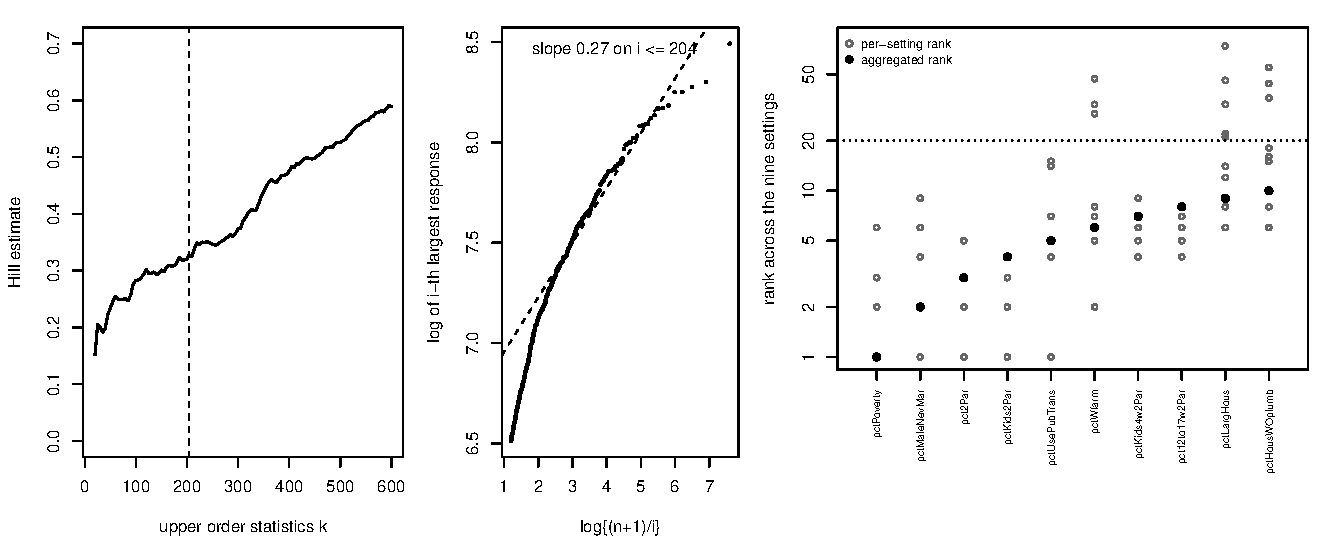
\includegraphics[width=.98\linewidth]{figures/crime_application.pdf}
\caption{Communities and Crime application ($n=1{,}993$, $p=99$,
$\alpha=n^{-0.3}$, $h=n^{-0.15}/2$). Left: Hill estimates for the
violent-crime rate; the dashed line marks the working level
$k=n\alpha=204$. Middle: Pareto QQ plot of the $600$ largest responses;
the dashed line is fitted over the working range $i\le204$. Right: for
the ten leading predictors of the aggregated screen, the nine
per-setting ranks (open circles) and the aggregated rank (filled
circles); the dotted line is the default retained size $d=20$.}
\label{fig:crime}
\end{figure}
